\chapter{Bearbeitung der Übungsaufgaben}

\section{Differenzenquotient}

Um die erste Ableitung $\frac{\mathrm{d}f}{\mathrm{d}x}(x)$ einer (hinreichend glatten) skalaren Funktion $f: \mathbb{R} \rightarrow \mathbb{R}$ an der Stelle $x$ numerisch zu approximieren kann man den rechtsseitigen (Gleichung(\ref{rechtsseitig})) und den zentralen (Gleichung(\ref{zentral})) Differenzenquotienten 

\begin{align}
	&\frac{\mathrm{d}f}{\mathrm{d}x}(x) = \frac{f(x+h)-f(x)}{h} + \mathcal{O}(h) \label{rechtsseitig}\\
	&\frac{\mathrm{d}f}{\mathrm{d}x}(x) = \frac{f(x+h)-f(x-h)}{2h} + \mathcal{O}
	\label{zentral}
\end{align}

nutzen wobei die Schrittweite $h \neq 0$ aber doch sehr klein zu wählen ist. Mit Hilfe der Taylorentwicklung mit Restgliedabschätzung wird im folgenden die Konvergenzordnung der obigen Differenzenquotienten ermittelt. An der Stelle $f(x+h)$ lautet allgemein das Taylorpolynom zweiten Grades 

\begin{equation*}
	T_2f(x+h)= f(x) +f'(x)h +\frac{f''(\xi)}{2!}h^2
\end{equation*}

mit der Fehlerabschätzung $f''(\xi)$ an einer unbekannten Stelle $\xi$ mit $ x <\xi <(x+h)$. Diese Gleichung umgestellt nach der gesuchten ersten Ableitung $f'(x)$ ergibt 

\begin{equation}
	f'(x) = \frac{f(x+h)-f(x)}{h}-\frac{f''(\xi)}{2}h
	\label{mitFehler}
\end{equation}

und mit oberer Abschätzung für den Fehler folgt 

\begin{equation}
	f'(x) = \frac{f(x+h)-f(x)}{h}+\mathcal{O}(h)
	\label{ohneFehler}
\end{equation}

wobei hier jetzt ersichtlich wird, dass die Korrektur des rechtseitigen Differenzenquotienten linear abhängig zur Schrittweite $h$ ist und somit eine Konvergenz 1. Ordnung hat. Konvergenz 1.Ordnung heißt in diesem Fall dass durch eine halbierung der Schrittweite $h$ auch die Fehlerabweichung halbiert wird.\\
Aus den Taylorpolynomen dritten Grades an den Stellen $f(x+h)$ (siehe Gleichung (\ref{(x+h)})) und $f(x-h)$(siehe Gleichung(\ref{(x-h)}))

\begin{align}
	&T_3f(x+h)= f(x) + f'(x)h +\frac{f''(x)}{2!}h^2 + \frac{f'''(\xi_r)}{3!}h^3
	\label{(x+h)}\\
	&T_3f(x-h)= f(x) - f'(x)h +\frac{f''(x)}{2!}h^2 - \frac{f'''(\xi_l)}{3!}h^3
	\label{(x-h)}
\end{align}

mit unbekannten $\xi_r$ und $\xi_l$, $(x-h) < \xi_l < x < \xi_r < (x+h)$ folgt nach den selben Schritten wie zuvor bei den Gleichungen (\ref{mitFehler}) und(\ref{ohneFehler}) 

\begin{equation*}
	f'(x) = \frac{f(x+h)-f(x-h)}{2h} + \mathcal{O}(h^2).
\end{equation*}

Der zentrale Differenzenquotient hat also eine Konvergenz 2. Ordnung, da die Korrektur quadratisch von der Schrittweite $h$ abhängt. Konvergenz zweiter Ordnung bedeutet dass bei einer halbierung der Schrittweite nur noch ein viertel des Fehlers gemacht wird.\\
Um einen Differenzenqoutient 4.Ordnung für die erste Ableitung zu konstruieren reichen nicht mehr nur zwei Punkte zum approximieren aus, stattdessen benötigt man jetzt 4 verschiedene Punkte $f(x-h)$, $f(x-\frac{h}{2})$, $f(x+\frac{h}{2})$ und $f(x+h)$ und kombiniert zwei zentrale Differenzenqotienten. Mit der selben Vorgehensweise wie zuvor lässt sich dann nachweisen dass der Differenzenquotient

\begin{equation*}
	\frac{\mathrm{d}f}{\mathrm{d}x}(x) = \frac{f(x+h)-f(x-h)+2f(x+\frac{h}{2})-2f(x-\frac{h}{2})}{4h}
\end{equation*}

von Konvergenz 4. Ordnung ist.\\

Um die Unterschiede der verschiedenen Differenzenquotienten graphisch darzustellen, bietet es sich an diese für verschieden große Schrittweiten $h$ sowie für verschiedene Funktionen zu testen. Getestet wird mit elf verschiedenen Schrittweiten $h \in [10^{-10},1]$ und den Funktion $f(x) = \exp(x+1)$ (siehe Abbildung \ref{fig:eFunktion}) an der Stelle $x=1$, $g(x) = \cos(x)$ (siehe Abbildung \ref{fig:cosinus}) an der Stelle $ x = \frac{\pi}{2}$ und 

\begin{equation}
	h(x)=
		 \begin{cases}
			6x^2+ 4 & x>1\\
			4x^3+6 & x\leq 1
		\end{cases}
	\label{polynom}
\end{equation}

an der Stelle $x=1$. Die geschriebene Octave-Routine (siehe Anhang!!!!) ermittelt den absoluten Fehler zwischen der tatsächlichen, analytisch bestimmten Ableitung der Funktionen und der numerischen Approximation mit den drei Differenzenquotienten. Zur Darstellung wird ein doppelt logarithmischer Plot verwendet (siehe Abbildungen \ref{fig:fehlerPlots}), da so sowohl die kleineren als auch die größeren Werte dargestellt werden können.\\
Auffällig ist, dass bei jeder der drei Testfunktionen die kleinste Schrittweite nicht die beste Annäherung liefert sondern es einen Tiefpunkt bei etwa $h=10^{-5}$ bzw $h=10^{-8}$ gibt. Das bedeutet dass ab diesem Punkt durch weiteres verkleinern der Schrittweite keine höhere Genauigkeit der Approximation erzielt werden kann. Außerdem erkennt man dass bei allen drei Verfahren die Fehler weitgehend ähnlich sind, mit Ausnahme der Approximation der Exponential-Funktion(\ref{fig:eFunktion}) mit dem rechtsseitigen Differenzenquotient, der hier deutlich schlechter abschneidet. Für Schrittweiten größer als die Ideale zeigen alle Graphen lineares Verhalten da hier, wie im Anschluss gezeigt wird, der Grad der Ordnung des numerischen Verfahrens zur Approximation ausschlaggebend ist für die Steigung. 
\begin{figure}[thbp]
	\centering
	\begin{subfigure}[tpbh]{0.68\textwidth}
		\centering
		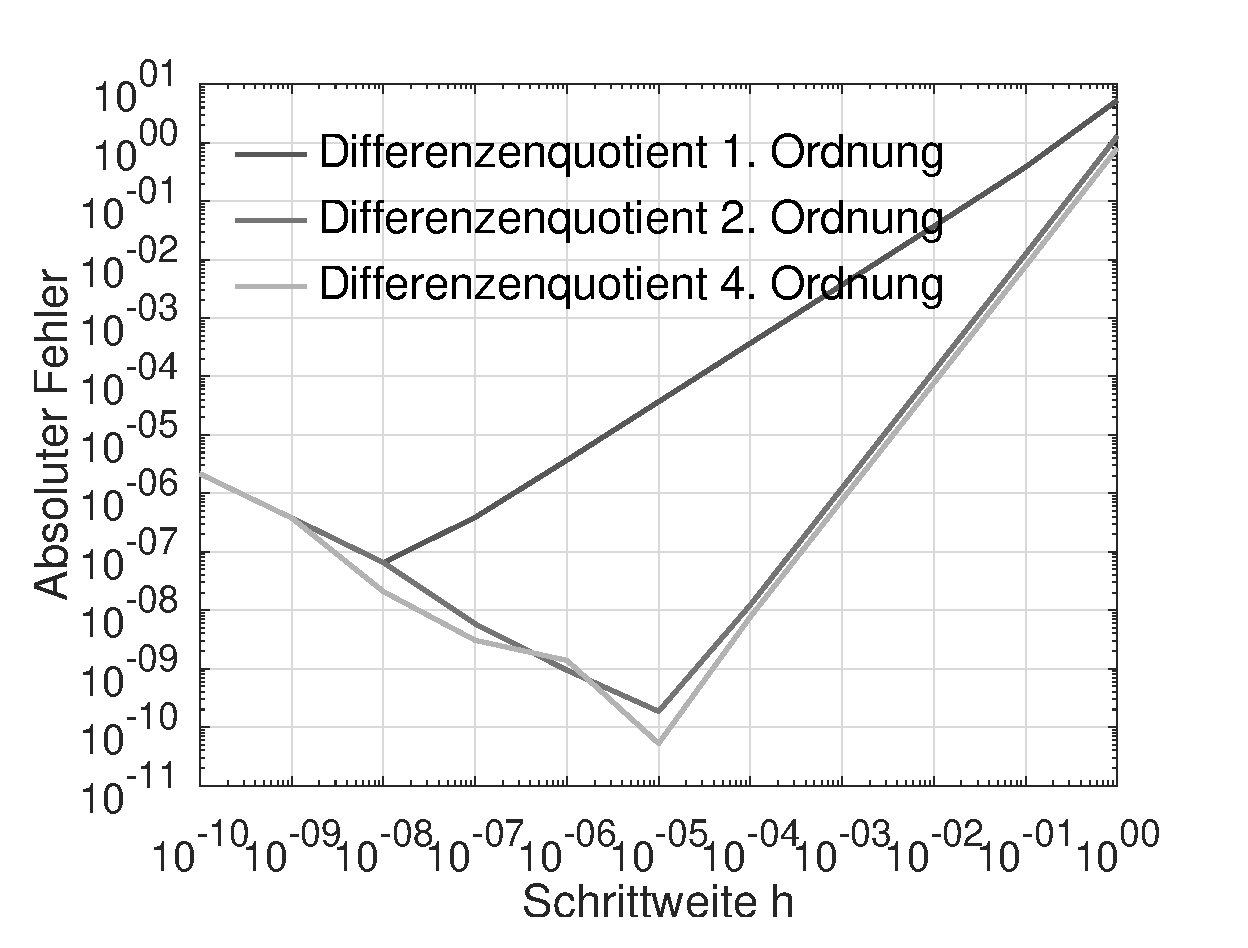
\includegraphics[width=\textwidth]{data/eFunktion}
		\caption{Fehler bei der Approximation von $f(x) = \exp(x+1)$ an der Stelle $x=1$}
		\label{fig:eFunktion}
	\end{subfigure}
	\begin{subfigure}[tpbh]{0.68\textwidth}
		\centering
		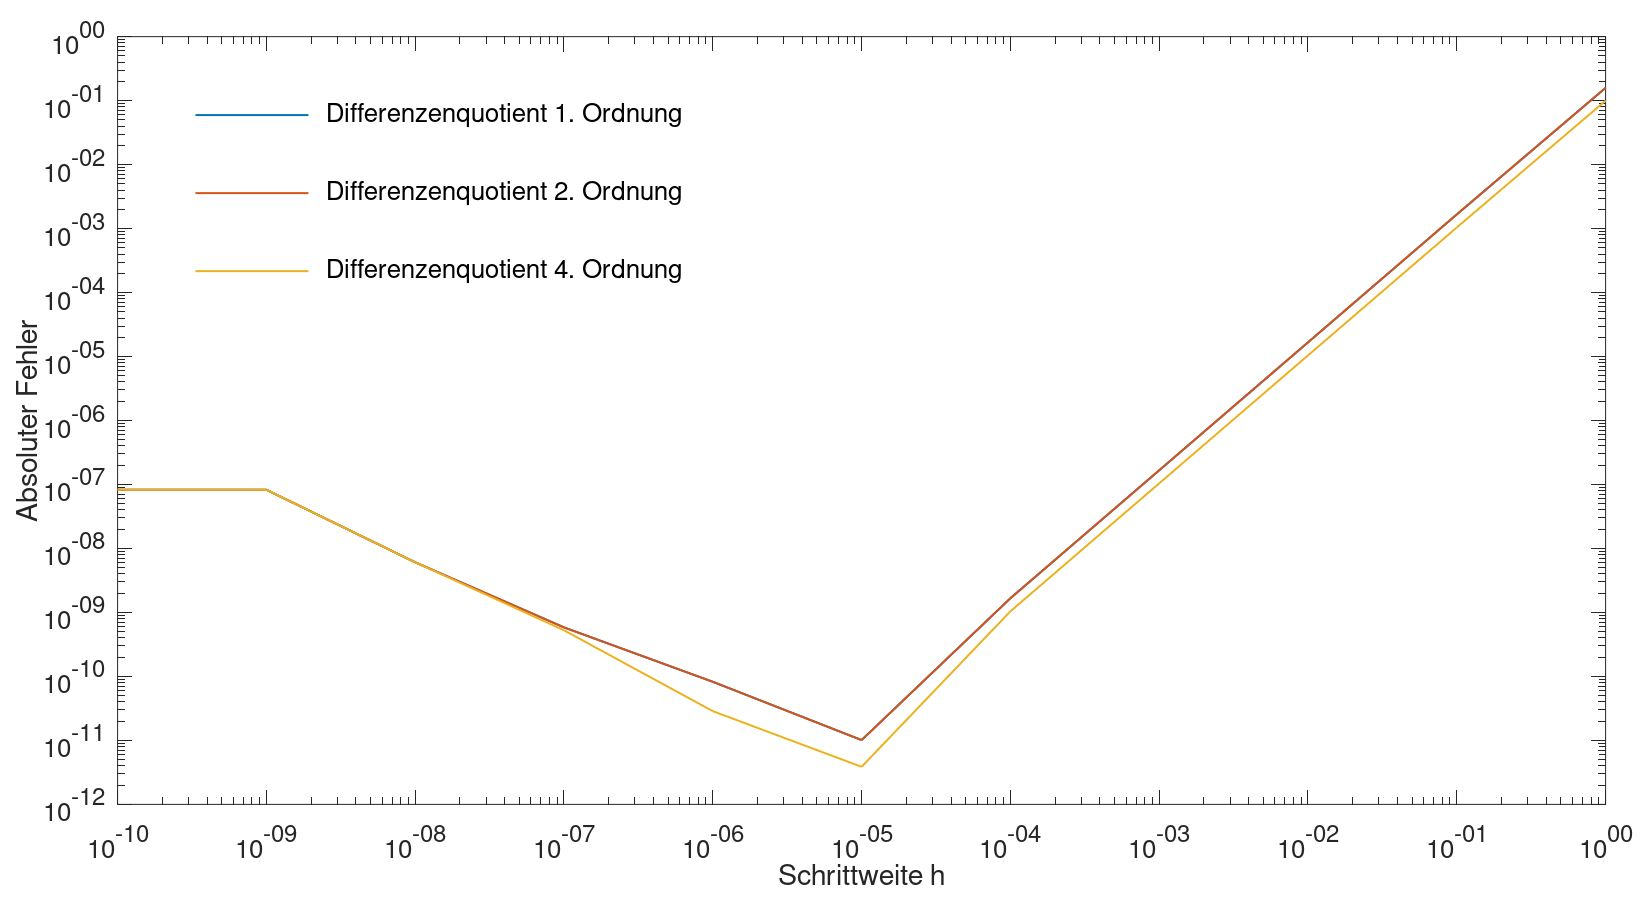
\includegraphics[width=\textwidth]{data/sinus}
		\caption{Fehler bei der Approximation von $g(x) = \cos(x)$ an der Stelle $x=\frac{\pi}{2}$}
		\label{fig:cosinus}
	\end{subfigure}
	\begin{subfigure}[tpbh]{0.68\textwidth}
		\centering
		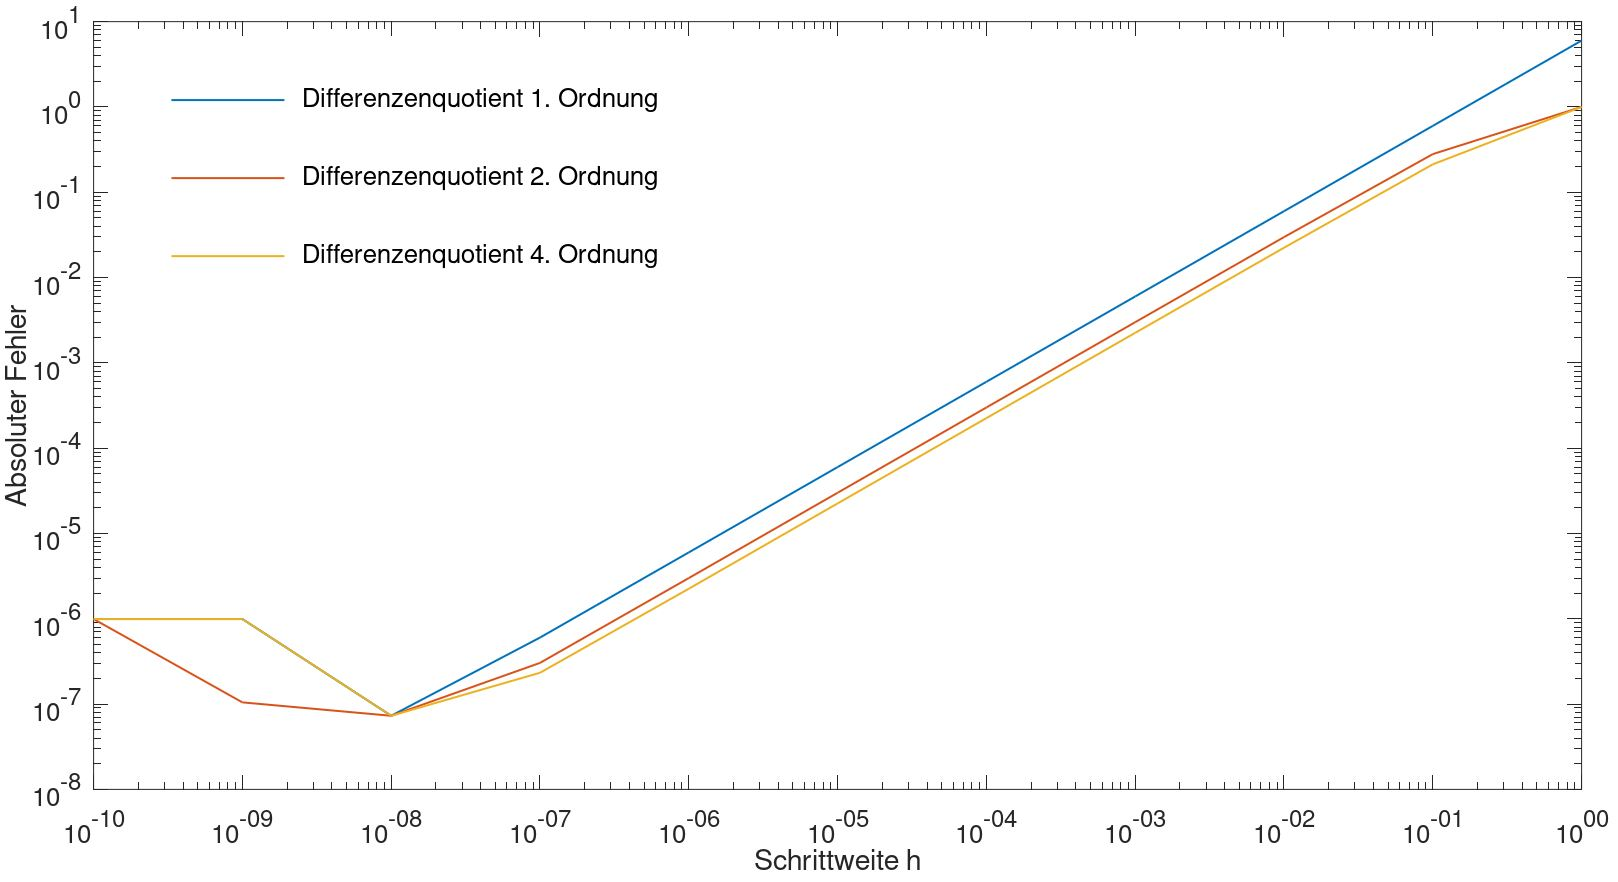
\includegraphics[width=\textwidth]{data/abschnittsFkt}
		\caption{Fehler bei der Approximation von Gleichung (\ref{polynom}) an der Stelle $x=1$ }
		\label{fig:Polynom}
	\end{subfigure}
	\caption{Fehler der numerischen Approximationen der ersten Ableitung in logarithmischem Koordinatensystem}
	\label{fig:fehlerPlots}
\end{figure}



Um in einem doppelt logarithmischem Koordinatensystem die Steigung einer Geraden zu berechnen (siehe Abbildung \ref{steigung}), reicht es nicht wie bei einem linearen Koordinatensystem die Werte $\Delta x$ und $\Delta y$ des allgemeinen Steigungsdreiecks durch die Differenz der auf den Achsen angegebenen Werte zu ermitteln.\\
Stattdessen wird auf die Werte die man an den jeweiligen Stellen auf den Achsen ablesen kann der Logarithmus zur selben Basis angewandt wie zur Erzeugung der logarithmischen Skala verwendet wurde, in diesem Beispiel zur Basis $10$. Der Quotient zur Ermittlung der Steigung lautet dann 

\begin{equation*}
	\frac{\Delta y}{\Delta x} = \frac{\log(C (10^{\Delta r +r})^p)-\log(C (10^r)^p)}{\log(10^{\Delta r +r}) - \log(10^r)}
\end{equation*} 

und unter Anwendung der Logarithmus Regeln $\log(u\cdot v) = \log u + \log v$ und $\log (10^w) = w$ 

\begin{equation*}
	\frac{\Delta y}{\Delta x} = \frac{(p(\Delta r +r)-pr)}{r+\Delta r -r}
	=p
\end{equation*}

Die Steigung der Fehlerabschätzung $\epsilon (h)$ist somit genau gleich mit der Ordnung $p$ des jeweiligen numerischen Verfahren zur Approximation.

\begin{figure}[htpb]
	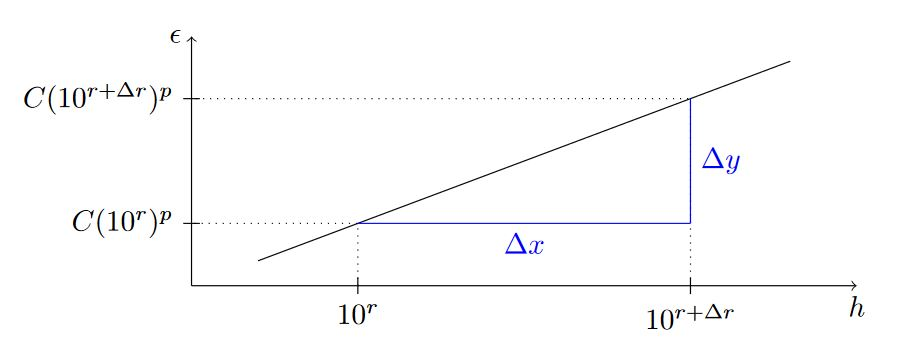
\includegraphics[width=\textwidth]{data/SteigungLogPlot}
	\caption{Allgemeines Steigungsdreieck in einem doppelt Logarithmischen Koordinatensystem}
	\label{steigung}
\end{figure}

Sollte das logarithmische Koordinatensystem nicht die Basis 10 haben sondern eine beliebige andere, ändert sich nichts an der Tatsache, dass die Steigung für $\epsilon (h)$ durch die Ordnung $p$ gegeben ist, da zur Berechnung des allgemeinen Steigungsdreiecks der Logarithmus zur selben beliebigen Basis auf alle Werte angewendet wird und somit unerheblich ist für die Steigung.





